\section{Uplink y métodos de acceso}\label{sec:ul}

En la subida, muchos UE comparten un mismo recurso y ninguno conoce a priori el estado de los demás. NR resuelve el acceso con dos mecanismos complementarios:
\begin{itemize}
  \item el \textbf{acceso aleatorio con contienda} por el PRACH, para el primer contacto o cuando se pierde la sincronización;
  \item el \textbf{acceso planificado} (\emph{grant-based}), en el que el gNB asigna explícitamente los recursos del PUSCH.
\end{itemize}

\subsection{Acceso aleatorio por PRACH}\label{sec:rach}
\subsubsection{Configuración del PRACH de la celda}
El SIB1 de la celda n78 difunde la configuración de la \cref{tab:prach}, tomada del log del gNB (ver la nota de la \cref{sec:gscn}). El \texttt{prach-ConfigurationIndex}~159 de la tabla~6.3.3.2-3 de TS~38.211 (FR1, espectro no apareado) corresponde a:
\begin{itemize}
  \item formato \textbf{B4};
  \item $n_\text{SFN}\bmod x = y$ con $x=1$, $y=0$: una ocasión en \emph{todas} las tramas;
  \item subtrama~9, símbolo inicial~0, 1 slot de PRACH por subtrama, 1 ocasión por slot y una duración de 12 símbolos.
\end{itemize}
Con $\Delta f_\text{RA}=30$~kHz y un solo slot de PRACH por subtrama, la ocasión cae en el segundo slot de la subtrama~9, es decir, en el \textbf{slot~19} de la trama (\cref{fig:tdd}). Coincide con lo observado en los logs del gNB (\cref{sec:crono}).

\begin{table}[htbp]
\centering
\caption{Parámetros del PRACH difundidos en el SIB1 de la celda n78.}
\label{tab:prach}
\begin{tabular}{lll}
\toprule
Parámetro & Valor & Significado \\
\midrule
\texttt{prach-ConfigurationIndex} & 159 & B4, subtrama 9, cada 10~ms, 12 símbolos \\
\texttt{msg1-SubcarrierSpacing} & 30~kHz & $L_\text{RA}=139$, $\mu=1$ \\
\texttt{msg1-FrequencyStart} & 11 & primer PRB del PRACH \\
\texttt{msg1-FDM} & 1 & una ocasión en frecuencia \\
\texttt{prach-RootSequenceIndex} (\texttt{l139}) & 1 & primera raíz lógica \\
\texttt{zeroCorrelationZoneConfig} & 0 & $N_\text{CS}=0$ (tabla 6.3.3.1-7) \\
preámbulos por SSB & 64 & con contienda \\
\texttt{preambleReceivedTargetPower} & $-100$~dBm & potencia objetivo inicial \\
\texttt{powerRampingStep} & 4~dB & escalón de rampa \\
\texttt{preambleTransMax} & 7 & intentos máximos \\
\texttt{ra-ResponseWindow} & 20 slots & 10~ms para recibir la RAR \\
\texttt{ra-ContentionResolutionTimer} & 64 subtramas & 64~ms para el Msg4 \\
\bottomrule
\end{tabular}
\end{table}

Según la tabla~6.3.3.2-1 de TS~38.211, un preámbulo de $L_\text{RA}=139$ con $\Delta f_\text{RA}=\Delta f_\text{PUSCH}=30$~kHz ocupa 12~PRB: el PRACH de la celda ocupa los PRB~11 a~22, en el centro de la portadora.

\subsubsection{Preámbulos Zadoff-Chu}
Los preámbulos son secuencias ZC de longitud 139 (\cref{eq:zc}) y sus desplazamientos cíclicos \cite[§6.3.3.1]{ts38211}:
\begin{equation}
x_{u,v}(n) = x_u\big((n + C_v)\bmod L_\text{RA}\big),\qquad C_v = v\,N_\text{CS}.
\end{equation}
Cada raíz $u$ da $\lfloor L_\text{RA}/N_\text{CS}\rfloor$ preámbulos ortogonales, siempre que el desplazamiento $N_\text{CS}$ supere el retardo de ida y vuelta más el delay spread. Si no alcanza, se toman raíces consecutivas hasta completar los 64. En esta celda $N_\text{CS}=0$ y cada raíz aporta \textbf{un único} preámbulo ($C_0=0$): los 64 preámbulos salen de 64 raíces distintas, a partir del índice lógico~1.

Esta configuración tiene dos consecuencias. Por un lado, no hay zona de correlación cero que limitar: el pico de correlación puede estar en cualquier lugar del período, y el radio de la celda no lo limita la secuencia (\cref{sec:ta}). Por otro lado, los preámbulos ya no son ortogonales entre sí, sino que tienen la correlación cruzada constante de $1/\sqrt{139}\approx -21$~dB entre raíces. En una celda con un puñado de UE, esto no es un problema.

\subsubsection{Formato B4: duración, CP y tiempo de guarda}
Para el formato B4 con $\mu=1$ y $\kappa=64$ \cite[tabla~6.3.3.1-2]{ts38211}:
\begin{align}
N_u &= 12\cdot 2048\,\kappa\, 2^{-\mu} = 786\,432\,T_c = 400{,}0~\mu\text{s},\\
N_\text{CP}^\text{RA} &= 936\,\kappa\, 2^{-\mu} = 29\,952\,T_c = 15{,}23~\mu\text{s}.
\end{align}
Como la ocasión empieza justo en el instante de 0,5~ms de la subtrama, TS~38.211 §5.3.2 le suma $16\kappa = 1024\,T_c$ al CP: $N_\text{CP}^\text{RA} = 30\,976\,T_c = 15{,}76~\mu$s, y el preámbulo dura $817\,408\,T_c = 415{,}8~\mu$s. Los 12 símbolos del slot que reserva la ocasión (el primero, con CP largo) duran
\begin{equation}
(65\,536 + 5632) + 11\cdot(65\,536 + 4608) = 842\,752\,T_c = 428{,}6~\mu\text{s}.
\end{equation}
La diferencia es un \textbf{tiempo de guarda implícito} de $842\,752 - 817\,408 = 25\,344\,T_c = 12{,}9~\mu$s.

\subsubsection{Procedimiento de 4 pasos}
El procedimiento con contienda (\cref{fig:rach}) se define en TS~38.321 §5.1 y TS~38.213 §8:
\begin{enumerate}
  \item \textbf{Msg1 (preámbulo).} El UE elige al azar uno de los 64 preámbulos y lo transmite en la próxima ocasión de PRACH asociada al SSB que mejor recibe. Todavía no tiene timing advance: transmite con $N_\text{TA}=0$.
  \item \textbf{Msg2 (RAR).} El gNB detecta el preámbulo, mide su retardo y responde por PDSCH, planificado con un PDCCH enmascarado con el RA-RNTI. El RA-RNTI identifica la ocasión en la que se envió el preámbulo \cite[§5.1.3]{ts38321}:
  \begin{equation}
  \text{RA-RNTI} = 1 + s_\text{id} + 14\,t_\text{id} + 14\cdot 80\,f_\text{id} + 14\cdot 80\cdot 8\,\text{ul\_carrier\_id}.
  \end{equation}
  En la celda, $s_\text{id}=0$, $t_\text{id}=19$, $f_\text{id}=0$ y el portador UL es el normal (0): $\text{RA-RNTI} = 1 + 14\cdot 19 = 267$. La RAR lleva el identificador del preámbulo detectado, el comando de TA, un \emph{grant} para el Msg3 y un identificador temporal (TC-RNTI). El UE la espera durante la \texttt{ra-ResponseWindow} (10~ms).
  \item \textbf{Msg3.} El UE aplica el TA y transmite en el PUSCH asignado un \texttt{RRCSetupRequest} con su identidad (parte del 5G-S-TMSI o un número aleatorio de 39~bits).
  \item \textbf{Msg4 (resolución de contienda).} El gNB responde con un \texttt{RRCSetup} y un MAC~CE \emph{UE Contention Resolution Identity}, que repite los primeros 48~bits del Msg3 recibido. El UE que reconoce su propio Msg3 ganó la contienda y convierte el TC-RNTI en su C-RNTI. Los demás vuelven a empezar.
\end{enumerate}

\begin{figure}[htbp]
\centering
\begin{tikzpicture}[font=\small,>=Stealth]
  \node[draw,fill=azul!15,minimum width=2.2cm] (ue) at (0,0) {UE};
  \node[draw,fill=naranja!15,minimum width=2.2cm] (gnb) at (8,0) {gNB};
  \draw[gris] (0,-0.35) -- (0,-6.6);
  \draw[gris] (8,-0.35) -- (8,-6.6);
  \draw[->,thick] (0,-0.9) -- node[above,midway]{\textbf{Msg1:} preámbulo ZC (PRACH, slot 19)} (8,-1.5);
  \node[right,align=left,font=\footnotesize] at (8.1,-1.5) {mide el retardo\\$\Rightarrow T_A$};
  \draw[->,thick] (8,-2.3) -- node[above,midway]{\textbf{Msg2:} RAR (RA-RNTI): $T_A$, grant, TC-RNTI} (0,-2.9);
  \node[left,align=right,font=\footnotesize] at (-0.1,-2.9) {aplica TA};
  \draw[->,thick] (0,-3.7) -- node[above,midway]{\textbf{Msg3:} RRCSetupRequest + identidad (PUSCH)} (8,-4.3);
  \draw[->,thick] (8,-5.1) -- node[above,midway]{\textbf{Msg4:} RRCSetup + Contention Resolution Id} (0,-5.7);
  \node[left,align=right,font=\footnotesize] at (-0.1,-5.7) {¿coincide?\\TC-RNTI$\to$C-RNTI};
  \draw[decorate,decoration={brace,amplitude=4pt,mirror},gris] (-1.9,-0.8) -- (-1.9,-3.0) node[midway,left=4pt,align=right,font=\footnotesize]{puede\\colisionar};
  \draw[decorate,decoration={brace,amplitude=4pt,mirror},gris] (-1.9,-3.6) -- (-1.9,-6.0) node[midway,left=4pt,align=right,font=\footnotesize]{resuelve la\\contienda};
\end{tikzpicture}
\caption{Procedimiento de acceso aleatorio de 4 pasos con contienda (TS~38.321 §5.1; TS~38.213 §8).}
\label{fig:rach}
\end{figure}

\subsubsection{Analogía con ALOHA ranurado}
El PRACH es un canal de acceso múltiple aleatorio, y su análisis es el de \textbf{ALOHA ranurado}:
\begin{itemize}
  \item las \textbf{ranuras} son las ocasiones de PRACH (en esta celda, una cada 10~ms, es decir, 100 por segundo);
  \item dentro de cada ranura hay 64 ``subcanales'' ortogonales o casi ortogonales: los preámbulos;
  \item una \textbf{colisión} ocurre cuando dos o más UE eligen el mismo preámbulo en la misma ocasión.
\end{itemize}
Para ALOHA ranurado con llegadas de Poisson y carga $G$ intentos por ranura, la probabilidad de éxito de un intento es $e^{-G}$ y el throughput, $S = Ge^{-G}$, con un máximo de $1/e\approx 0{,}368$ en $G=1$. Para ALOHA puro, $S = Ge^{-2G}$ (máximo $1/(2e)$), porque el período vulnerable es el doble \cite{tanenbaum}. En el PRACH, la carga se reparte entre 64 preámbulos: si $k$ UE acceden en la misma ocasión, la probabilidad de que un UE dado no colisione es
\begin{equation}
\Pr\{\text{sin colisión}\} = \left(1 - \frac{1}{64}\right)^{k-1},
\label{eq:colision}
\end{equation}
que vale 0,98 para $k=2$ y 0,54 para $k=40$ (\cref{fig:aloha}).

\begin{figure}[htbp]
\centering
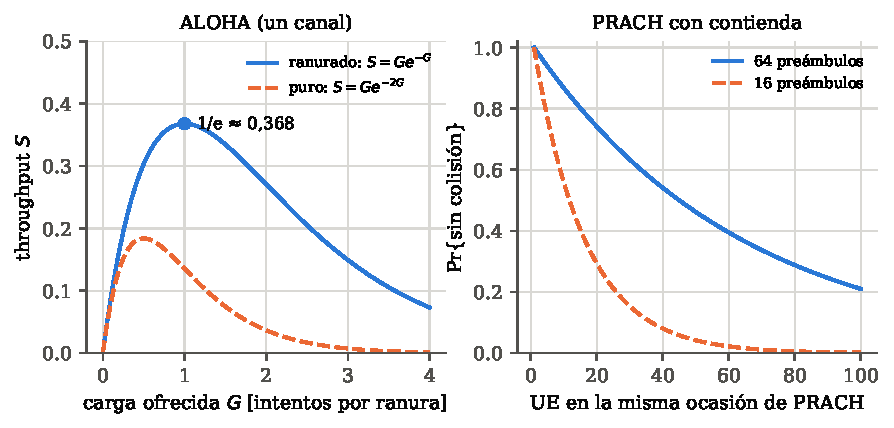
\includegraphics[width=\linewidth]{figuras/fig_aloha.pdf}
\caption{Izquierda: throughput de ALOHA ranurado y puro. Derecha: probabilidad de que un UE no colisione en una ocasión de PRACH, según la cantidad de UE que acceden en ella, con 64 y 16 preámbulos (\cref{eq:colision}).}
\label{fig:aloha}
\end{figure}

La diferencia con el ALOHA clásico está en \textbf{cómo se detecta y resuelve la colisión}. Dos UE que eligen el mismo preámbulo son indistinguibles para el gNB, que ve un solo pico de correlación (o dos picos cercanos) y responde con una sola RAR. Los dos UE creen haber sido escuchados y transmiten su Msg3 en el mismo grant: ahí sí colisionan. A lo sumo uno se decodifica (efecto captura) y el Msg4 lo identifica. El otro detecta que perdió al vencer el \texttt{ra-ContentionResolutionTimer} o al no reconocer su identidad, y reintenta tras un \emph{backoff} aleatorio, como en ALOHA. El costo de una colisión es, entonces, el tiempo de los cuatro mensajes, no solo una ranura.

\subsubsection{Power ramping}
El UE no conoce de antemano la potencia necesaria y la estima en lazo abierto \cite[§7.4]{ts38213}:
\begin{equation}
P_\text{PRACH} = \min\left\{P_\text{CMAX},\; P_\text{PRACH,target} + PL\right\}~[\text{dBm}],
\label{eq:pprach}
\end{equation}
donde $PL$ es la pérdida de trayecto estimada con el SSB, y la potencia objetivo, fijada por la MAC, crece en cada reintento \cite[§5.1.3]{ts38321}:
\begin{equation}
P_\text{PRACH,target} = \texttt{preambleReceivedTargetPower} + \Delta_\text{PREAMBLE} + (n-1)\cdot\texttt{powerRampingStep}.
\label{eq:ramping}
\end{equation}
Para el formato B4, $\Delta_\text{PREAMBLE} = 3\mu = 3$~dB \cite[tabla~7.3-2]{ts38321}. En la celda, el primer intento apunta a $-100 + 3 = -97$~dBm en el receptor del gNB, y el séptimo y último, a $-97 + 6\cdot 4 = -73$~dBm. Si se agota \texttt{preambleTransMax} sin RAR, la MAC informa un problema de acceso aleatorio a RRC. El escalonamiento evita que todos los UE transmitan con la máxima potencia, lo que aumentaría la interferencia y el consumo. Cada UE se acerca desde abajo a la potencia justa.

\subsubsection{Timing advance y radio de cobertura}\label{sec:ta}
Como la señal tarda $d/c$ en llegar al UE y otro tanto en volver, un UE a distancia $d$ que transmitiera alineado con la bajada que recibe llegaría al gNB con un retraso de $2d/c$. Para que las transmisiones de todos los UE lleguen alineadas a la grilla del gNB (y se conserve la ortogonalidad entre ellos), cada UE adelanta su trama de subida en \cite[§4.3.1]{ts38211}
\begin{equation}
T_\text{TA} = (N_\text{TA} + N_\text{TA,offset})\,T_c.
\label{eq:tta}
\end{equation}
$N_\text{TA,offset}$ es un adelanto fijo que deja tiempo de conmutación al gNB. En FR1 sin coexistencia LTE-NR vale $25\,600\,T_c\approx 13~\mu$s, y es el valor por defecto en FR1 cuando la red no señaliza \texttt{n-TimingAdvanceOffset} \cite[§7.1.2, tabla~7.1.2-2]{ts38133}. $N_\text{TA}$ compensa la ida y vuelta:
\begin{equation}
N_\text{TA}\,T_c = \frac{2d}{c}\quad\Longrightarrow\quad d = \frac{c\,N_\text{TA}\,T_c}{2}.
\label{eq:ta_d}
\end{equation}

\paragraph{Paso del TA.} Para una SCS de $2^\mu\cdot 15$~kHz, el comando de TA se expresa en múltiplos de $16\cdot 64\,T_c/2^\mu$ \cite[§4.2]{ts38213}. Con $\mu=1$:
\begin{equation}
\Delta T_\text{TA} = \frac{16\cdot 64}{2}\,T_c = 512\,T_c = 0{,}260~\mu\text{s}
\;\Rightarrow\;
\Delta d = \frac{c\,\Delta T_\text{TA}}{2} = \frac{3\cdot 10^8\cdot 0{,}260\cdot 10^{-6}}{2} \approx 39~\text{m}.
\end{equation}
\begin{itemize}
  \item \textbf{En la RAR}, el TA es absoluto: $T_A\in\{0,\dots,3846\}$ y $N_\text{TA} = T_A\cdot 16\cdot 64/2^\mu$ \cite[§4.2]{ts38213}. El máximo es $3846\cdot 0{,}260~\mu\text{s} = 1{,}0016$~ms, que corresponde a $d_\text{max}\approx 150$~km.
  \item \textbf{En la conexión}, el MAC~CE \emph{Timing Advance Command} es relativo: $N_\text{TA,new} = N_\text{TA,old} + (T_A-31)\cdot 16\cdot 64/2^\mu$, con $T_A\in\{0,\dots,63\}$, es decir, correcciones de $-31$ a $+32$ pasos.
\end{itemize}

\paragraph{El alcance geométrico lo limita el PRACH, no el TA.} Los 150~km que admite el campo de la RAR son una cota de señalización. La limitación física aparece \emph{antes} de que exista un TA: el preámbulo se transmite con $N_\text{TA}=0$ y llega al gNB con un retraso $2d/c$. Para que se lo pueda detectar sin interferir con lo que sigue tienen que cumplirse dos condiciones:
\begin{enumerate}
  \item el retardo más el delay spread tiene que caber en el CP del preámbulo, para que la ventana de correlación del gNB contenga un período completo de la secuencia: $2d/c + \tau_\text{max} \le T_\text{CP}^\text{RA}$;
  \item el preámbulo retrasado no tiene que invadir los símbolos siguientes: $2d/c \le T_\text{GT}$.
\end{enumerate}
Para el formato B4 con $\mu=1$:
\begin{align}
\text{por el CP:}\quad & d \le \frac{c\,T_\text{CP}^\text{RA}}{2} = \frac{3\cdot 10^8\cdot 15{,}76\cdot 10^{-6}}{2} \approx 2{,}36~\text{km}\quad(\tau_\text{max}=0),\\
\text{por la guarda:}\quad & d \le \frac{c\,T_\text{GT}}{2} = \frac{3\cdot 10^8\cdot 12{,}9\cdot 10^{-6}}{2} \approx 1{,}9~\text{km}.
\end{align}
El alcance geométrico de la configuración es, entonces, del orden de \textbf{2~km}. Es una cota temporal orientativa, calculada por el grupo sobre los valores de la norma, que no incluye el presupuesto de enlace, la sensibilidad ni la interferencia (el alcance radioeléctrico no se midió): si los símbolos 12 y 13 del slot~19 no se usan para otras transmisiones de subida, la guarda real es mayor y manda el límite del CP. Por eso los formatos largos ($L_\text{RA}=839$, con CP de hasta $\approx 684~\mu$s en el formato~1) se reservan para celdas de decenas de kilómetros, y los cortos, como el B4, para celdas chicas. En la jaula de Faraday, con distancias de metros, el TA inicial es prácticamente 0: lo que importa es su \emph{evolución} (\cref{sec:crono}).

Una vez conectado, el gNB mide continuamente el retardo de las señales de subida (DM-RS, SRS, PUCCH) y envía correcciones relativas. El CP de los símbolos de datos (2,34~$\mu$s) solo tiene que absorber el delay spread y el error residual de TA. El TA \emph{no} lo cubre.

\subsection{Acceso planificado (grant-based)}\label{sec:grant}
Una vez conectado, el UE no transmite datos cuando quiere. El gNB es el que asigna cada PUSCH:
\begin{enumerate}
  \item \textbf{Scheduling Request (SR).} Cuando llegan datos al buffer y el UE no tiene grant, envía un SR por el PUCCH, un pedido de un bit en recursos periódicos dedicados \cite[§5.4.4]{ts38321}, \cite[§9.2.4]{ts38213}.
  \item \textbf{Grant inicial.} El gNB responde con un DCI~0\_0 o 0\_1 en el PDCCH, que asigna PRB, MCS, proceso HARQ y el desfase $k_2$ entre el DCI y el PUSCH \cite[§6.1.2.1]{ts38214}. En el SIB1 de la celda, la tabla de asignación temporal común del PUSCH tiene $k_2\in\{4,5,6,7,11\}$ slots.
  \item \textbf{Buffer Status Report (BSR).} En ese primer PUSCH, el UE incluye un MAC~CE BSR con la cantidad de datos pendientes por grupo de canales lógicos \cite[§5.4.5]{ts38321}. Con esa información, el gNB dimensiona los grants siguientes.
  \item \textbf{Transmisión y HARQ.} El gNB decodifica cada PUSCH y, si falla, pide una retransmisión con otro DCI (HARQ asíncrono, hasta 16 procesos).
\end{enumerate}
El ciclo SR $\to$ grant $\to$ PUSCH le agrega latencia a la subida. En TDD, el SR solo se puede enviar en un slot de subida, el grant llega en uno de bajada, y el PUSCH vuelve a necesitar un slot de subida al menos $k_2\ge 4$ slots después. Esta es una de las causas de la asimetría y la latencia medidas (\cref{sec:resultados}).

Para reducir esa latencia, NR prevé el \textbf{configured grant} \cite[§5.8.2]{ts38321}: recursos de PUSCH periódicos preasignados que el UE usa sin pedirlos. El de tipo~1 se configura completo por RRC; el de tipo~2 se configura por RRC y se activa o desactiva con un DCI. Es la base de URLLC. En esta celda no se usó.

\subsection{Qué pasa cuando el celular está callado}\label{sec:callado}
Mantener al UE escuchando el PDCCH en todos los slots consume batería. NR escalona los estados según la actividad:
\begin{itemize}
  \item \textbf{DRX en RRC\_CONNECTED} \cite[§5.7]{ts38321}: el UE monitorea el PDCCH solo durante el \emph{on duration} de cada ciclo DRX (corto o largo). Cada vez que recibe un DCI con datos nuevos, arranca el \texttt{drx-InactivityTimer} y se queda despierto mientras haya actividad. Al vencer, vuelve al ciclo. El costo es latencia: un paquete que llega mientras el UE duerme espera al siguiente \emph{on duration}.
  \item \textbf{Paso a RRC\_INACTIVE o RRC\_IDLE} \cite[§4.2.1]{ts38331}: después de un período sin tráfico (temporizador de inactividad del gNB), la red libera la conexión con un \texttt{RRCRelease}. En RRC\_INACTIVE, el UE y la red guardan el contexto (seguridad, configuración) y la reanudación es rápida (\texttt{RRCResumeRequest}). En RRC\_IDLE se pierde el contexto de acceso radio y hay que volver a establecer la conexión.
  \item \textbf{Paging} \cite{ts38304}: en INACTIVE o IDLE, el UE se despierta solo en su \emph{paging occasion}, una vez por ciclo de paging (en la celda, 128 tramas = 1,28~s). Si la red tiene datos para él, lo llama por el PDCCH con el P-RNTI, y el UE inicia el acceso aleatorio.
  \item \textbf{Vencimiento del temporizador de TA} \cite[§5.2]{ts38321}: el TA que mantiene el gNB solo es válido mientras el UE se mueve poco. Si no recibe comandos de TA durante \texttt{timeAlignmentTimer}, el UE considera que perdió el sincronismo de subida: vacía los buffers HARQ, libera el PUCCH, el SRS y los configured grants, y \textbf{para volver a transmitir tiene que pasar otra vez por el RACH}. En la celda, \texttt{timeAlignmentTimerCommon} = \texttt{infinity} en el SIB1.
\end{itemize}

\subsection{CP-OFDM contra DFT-s-OFDM}\label{sec:dfts}
\subsubsection{Las dos formas de onda de la subida}
En la bajada, NR usa siempre CP-OFDM. En la subida admite dos formas de onda: CP-OFDM (sin precodificación por transformada) y \textbf{DFT-s-OFDM}, que se activa con \texttt{transformPrecoder} \cite[§6.3.1.4]{ts38211}. DFT-s-OFDM (equivalente al SC-FDMA de LTE) antepone a la IFFT una DFT de $M$ puntos sobre los símbolos de modulación de cada símbolo OFDM:
\begin{equation}
y(l\,M_\text{sc}^\text{PUSCH} + k) = \frac{1}{\sqrt{M_\text{sc}^\text{PUSCH}}}\sum_{i=0}^{M_\text{sc}^\text{PUSCH}-1} \tilde{x}(l\,M_\text{sc}^\text{PUSCH}+i)\,e^{-j\frac{2\pi i k}{M_\text{sc}^\text{PUSCH}}},
\label{eq:transform}
\end{equation}
con la restricción \cite[§6.3.1.4]{ts38211}
\begin{equation}
M_\text{sc}^\text{PUSCH} = 12\cdot 2^{\alpha_2}\cdot 3^{\alpha_3}\cdot 5^{\alpha_5},
\label{eq:235}
\end{equation}
que asegura que la DFT tenga solo factores primos chicos y se pueda calcular eficientemente. Hay una consecuencia práctica: \textbf{51~PRB no está permitido} ($51 = 3\cdot 17$), así que con DFT-s-OFDM el gNB asignó como máximo 50~PRB ($50 = 2\cdot 5^2$). Así se observó en la prueba A/B/A (\cref{sec:crono}). La transformación solo se admite con una capa.

\begin{figure}[htbp]
\centering
\begin{tikzpicture}[font=\footnotesize,>=Stealth,
  b/.style={draw,rounded corners=2pt,minimum height=0.75cm,align=center,fill=white},
  dft/.style={b,fill=naranja!20},
  eq/.style={b,fill=verde!20}]
  % Transmisor
  \node[font=\small\bfseries,anchor=west] at (-0.4,1.0) {Transmisor (UE)};
  \node[b] (mod) at (0.6,0) {Modulación\\QAM};
  \node[dft] (dftb) at (2.7,0) {DFT\\$M$ puntos};
  \node[b] (map) at (4.9,0) {Mapeo a\\$M$ subport.};
  \node[b] (ifft) at (7.0,0) {IFFT\\$N$ puntos};
  \node[b] (cp) at (9.0,0) {+CP};
  \node[b] (rf) at (10.7,0) {DAC/RF\\PA};
  \draw[->] (mod) -- (dftb); \draw[->] (dftb) -- (map); \draw[->] (map) -- (ifft); \draw[->] (ifft) -- (cp); \draw[->] (cp) -- (rf);
  % Receptor
  \node[font=\small\bfseries,anchor=west] at (-0.4,-1.3) {Receptor (gNB)};
  \node[b] (rrf) at (10.7,-2.3) {RF/ADC};
  \node[b] (rcp) at (9.0,-2.3) {$-$CP};
  \node[b] (fft) at (7.0,-2.3) {FFT\\$N$ puntos};
  \node[b] (dem) at (4.9,-2.3) {Demapeo\\$M$ subport.};
  \node[eq] (equ) at (2.7,-2.3) {Ecualización\\por subport.};
  \node[dft] (idft) at (0.6,-2.3) {IDFT\\$M$ puntos};
  \node[b] (det) at (0.6,-3.7) {Demodulación\\QAM};
  \draw[->] (rrf) -- (rcp); \draw[->] (rcp) -- (fft); \draw[->] (fft) -- (dem); \draw[->] (dem) -- (equ); \draw[->] (equ) -- (idft); \draw[->] (idft) -- (det);
  \node[eq,font=\scriptsize] (ce) at (4.9,-3.7) {Estimación de canal\\(DM-RS ZC en frecuencia)};
  \draw[->] (ce) -| (equ);
\end{tikzpicture}
\caption{Cadenas de DFT-s-OFDM. Los bloques naranjas (DFT/IDFT de $M$ puntos) son los que la diferencian de CP-OFDM: sin ellos, la cadena es la de CP-OFDM, y el ecualizador entrega directamente símbolos QAM. En verde, la ecualización en frecuencia, que va después de la FFT y del demapeo, y antes de la IDFT.}
\label{fig:dfts}
\end{figure}

\subsubsection{Por qué baja la PAPR}
Con mapeo localizado (subportadoras contiguas), la cadena DFT~$M$ $\to$ IFFT~$N$ equivale a interpolar los $M$ símbolos de modulación con un núcleo tipo sinc periódica. La señal en el tiempo es, en esencia, \textbf{una portadora única} que recorre los símbolos de la constelación uno tras otro. Su envolvente sigue, en los instantes de los símbolos, a la constelación (QPSK tiene allí amplitud constante); entre ellos, la interpolación genera picos moderados. La PAPR depende sobre todo de la modulación y mucho menos de $M$ que en CP-OFDM, donde cada muestra es la suma aproximadamente gaussiana de la \cref{sec:papr}.

La simulación ilustrativa de la \cref{fig:papr} (derecha), con 612 subportadoras en una FFT de 768, da al nivel $10^{-3}$:
\begin{itemize}
  \item CP-OFDM: $\approx 11{,}6$~dB, prácticamente igual con QPSK, 16QAM o 256QAM;
  \item DFT-s-OFDM: 7,9~dB con QPSK, 8,9~dB con 16QAM y 9,2~dB con 256QAM.
\end{itemize}
En esa simulación, la ventaja es de 2,5 a 3,7~dB, mayor cuanto más simple es la modulación. No es una medición del teléfono. Para el UE eso significa un back-off menor: con el mismo amplificador puede transmitir más potencia media (la norma le permite una reducción de potencia máxima, MPR, menor con DFT-s-OFDM: con QPSK, hasta 1~dB contra hasta 3~dB de CP-OFDM en las asignaciones de borde y externas \cite[§6.2.2, tabla~6.2.2-1]{ts38101}), o la misma potencia con más eficiencia.

\subsubsection{Cuándo conviene cada una}
\begin{itemize}
  \item \textbf{DFT-s-OFDM:} conviene cuando el UE está \textbf{limitado en potencia}, en el borde de la celda, donde el amplificador ya trabaja cerca de saturación y cada dB de back-off se traduce en alcance o en SINR. En ese régimen se usan modulaciones bajas (incluida $\pi/2$-BPSK, que solo existe con transform precoding), justo donde la ventaja de PAPR es mayor.
  \item \textbf{CP-OFDM:} conviene con \textbf{SINR alta} y potencia sobrante. Admite MIMO de varias capas, asignaciones de PRB no contiguas y cualquier cantidad de PRB, y cada subportadora conserva su propia SINR después de ecualizar. En canales selectivos en frecuencia y con MCS altos, suele rendir más.
\end{itemize}
Por eso el gNB puede cambiar de forma de onda según las condiciones del UE (la conmutación dinámica llegó en releases posteriores). En la prueba de la \cref{sec:crono}, con una SINR media de $\approx 27$~dB y el UE muy cerca de la antena, DFT-s-OFDM no mejoró el throughput, lo que es coherente con este análisis si el UE no estaba limitado en potencia.

\subsubsection{Dónde se ecualiza en DFT-s-OFDM}\label{sec:ecualizacion}
En el receptor (\cref{fig:dfts}), la ecualización se hace \textbf{en frecuencia, después de la FFT de $N$ puntos y del demapeo de las $M$ subportadoras, y antes de la IDFT de $M$ puntos} que deshace la precodificación. La justificación es la siguiente:
\begin{enumerate}
  \item Gracias al CP, después de la FFT el canal es \textbf{diagonal en frecuencia}: en cada subportadora, $R_k = H_k Y_k + W_k$. Un ecualizador de un coeficiente por subportadora (ZF $1/H_k$, o MMSE $H_k^*/(|H_k|^2+\sigma^2)$) invierte el canal con complejidad mínima, igual que en CP-OFDM. La DM-RS del PUSCH con DFT-s-OFDM se mapea directamente en frecuencia (una secuencia ZC de baja PAPR, sin precodificar), así que da $H_k$ en el mismo dominio.
  \item Después de la IDFT, cada muestra es una combinación de \emph{todas} las subportadoras, cada una afectada por un $H_k$ distinto: el canal deja de ser diagonal y aparece interferencia entre símbolos. Ecualizar ahí exigiría un ecualizador en el tiempo de muchos coeficientes, que es justamente lo que el CP permite evitar.
  \item La IDFT reparte el error residual y el ruido de forma pareja entre los $M$ símbolos, así que un desvanecimiento profundo en algunas subportadoras degrada un poco a todos los símbolos en lugar de borrar algunos. Es un promediado en frecuencia: el MMSE da una SINR efectiva única para toda la asignación. En CP-OFDM también se usa un único MCS por asignación, pero el decodificador LDPC recibe la confiabilidad propia de cada subportadora; en DFT-s-OFDM, el ruido realzado de las subportadoras débiles se reparte entre todos los símbolos. Por eso, en canales muy selectivos y con MCS altos, DFT-s-OFDM suele rendir algo menos.
\end{enumerate}
En CP-OFDM no hay IDFT de $M$ puntos: el ecualizador entrega directamente los símbolos de cada subportadora al demodulador.

\subsection{Control de potencia del PUSCH y PHR}\label{sec:potencia_ul}
A diferencia de la bajada, en la subida cada UE controla su propia potencia. Hay tres motivos:
\begin{itemize}
  \item el \textbf{efecto cerca-lejos}: los UE cercanos no deben tapar a los lejanos en el receptor del gNB;
  \item la \textbf{interferencia} hacia las celdas vecinas;
  \item la \textbf{batería}.
\end{itemize}
La potencia del PUSCH en la ocasión $i$ es \cite[§7.1.1]{ts38213}
\begin{equation}
P_\text{PUSCH}(i) = \min\left\{
\begin{aligned}
&P_\text{CMAX}(i),\\
&P_\text{O\_PUSCH}(j) + 10\log_{10}\!\left(2^{\mu}\, M_\text{RB}^\text{PUSCH}(i)\right) + \alpha(j)\cdot PL(q_d) + \Delta_\text{TF}(i) + f(i,l)
\end{aligned}
\right\}~[\text{dBm}],
\label{eq:ppusch}
\end{equation}
donde:
\begin{itemize}
  \item $P_\text{CMAX}$: potencia máxima configurada del UE, 23~dBm para la clase de potencia~3 \cite[§6.2.1]{ts38101}, menos las reducciones permitidas (MPR);
  \item $P_\text{O\_PUSCH} = P_\text{O\_NOMINAL\_PUSCH} + P_\text{O\_UE\_PUSCH}$: densidad de potencia objetivo en el receptor, por RB de 15~kHz. En la celda, \texttt{p0-NominalWithGrant} = $-76$~dBm;
  \item $10\log_{10}(2^\mu M_\text{RB})$: escala la potencia con el ancho asignado. El factor $2^\mu$ convierte RB de $2^\mu\cdot 15$~kHz a RB de 15~kHz, para que $P_\text{O}$ sea una densidad independiente de la numerología;
  \item $\alpha\cdot PL$: compensación \emph{fraccional} de la pérdida de trayecto ($0\le\alpha\le 1$). Con $\alpha<1$, los UE del borde compensan solo una parte de su pérdida, lo que limita la interferencia hacia otras celdas a costa de su propia SINR. $PL$ se estima como \texttt{ss-PBCH-BlockPower} menos la RSRP filtrada;
  \item $\Delta_\text{TF}$: corrección por formato de transporte (bits por RE), que da más potencia a los MCS más exigentes cuando está habilitada;
  \item $f(i,l)$: el término de \textbf{lazo cerrado}, que acumula los comandos TPC enviados en los DCI. Corrige los errores del lazo abierto, como el sesgo de $PL$ por la potencia no calibrada de la B210 (\cref{sec:potencia_dl}).
\end{itemize}

\paragraph{Ejemplo ilustrativo.} No se midió la pérdida de trayecto: el siguiente cálculo solo ilustra los órdenes de magnitud. Con $\alpha=1$, $PL = 60$~dB, $\mu=1$, $M_\text{RB}=51$ y $\Delta_\text{TF}=f=0$,
\begin{equation}
P_\text{PUSCH} = -76 + 10\log_{10}(2\cdot 51) + 60 = -76 + 20{,}1 + 60 = 4{,}1~\text{dBm} < 23~\text{dBm}.
\end{equation}
En este ejemplo hipotético, el UE tendría casi 19~dB de margen: estaría lejos de la saturación y la menor PAPR de DFT-s-OFDM no le aportaría nada. Que el Redmi estuviera en una situación así durante la prueba es una hipótesis, que solo el PHR puede confirmar.

\paragraph{Power headroom report (PHR).} El margen se informa al gNB en un MAC~CE \cite[§5.4.6]{ts38321}, \cite[§7.7]{ts38213}:
\begin{equation}
PH(i) = P_\text{CMAX}(i) - \left\{P_\text{O\_PUSCH} + 10\log_{10}(2^\mu M_\text{RB}) + \alpha\,PL + \Delta_\text{TF} + f\right\}~[\text{dB}].
\label{eq:phr}
\end{equation}
Un PH positivo indica que el UE puede recibir más PRB o un MCS más alto; uno negativo, que está limitado en potencia y que el gNB debería reducir la asignación o, si está configurado, pasar a DFT-s-OFDM. Registrar el PHR es justamente lo que faltó para confirmar la interpretación de la prueba de DFT-s-OFDM (\cref{sec:trabajo_futuro}).
